\chapter{Application Architecture and its Implementation}

In the Figure \ref{f-screenSmallModule} you can see the print screen of the running application. The whole window system (window, menus, etc.) is provided by Netbeans platform. On the left side (number 1) you can see the project tree, which is the standard component of Netbeans platform (frequently used e.g. in Netbeans IDE). Next to the project tree there is a workspace (number 2) where user can create and manage his/her class model. On the right side there is a panel (number 3), called Tool Chooser, which is used for tool selection (tool for new class addition, etc.).

\begin{figure}[!ht]
\begin{center}
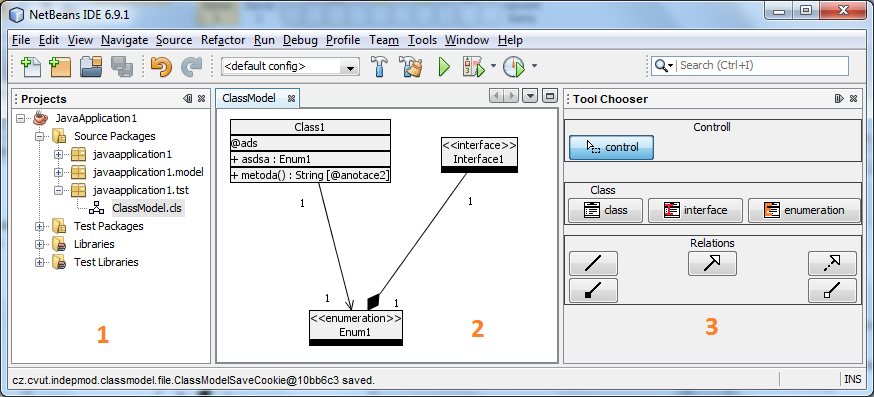
\includegraphics[width=\textwidth]{img/screenSmall.png}
\caption{Screenshot of the program}
\label{f-screenSmallModule}
\end{center}
\end{figure}

Indepmod Class Notation plugin consists of several modules which provides its functionality. The plugin is divided into modules because some parts (e.g. API of the plugin) should be public and some parts shouldn't. Public module means that it can be used in other plugins (or other modules of a plugin). This module division helps to comply with rules of loose coupling and high cohesion. These modules are:

\begin{itemize}
	\item Editor - the main module of the Indepmod Class Notation plugin. This module takes care about whole class modeling. It handles the workspace and its user interface can be seen in the Figure \ref{f-screenSmallModule} between Project Tree and Tool Chooser panels. The workspace has a JGraph inside which controls whole class modeling.
    \item API - this module provides a public API (interfaces). Implementations of these interfaces can be found (e.g. by other Netbeans plugins) in the Lookup of the workspace (part of the Editor module). This module is public so it can be used (imported as a library) by any other plugin.
    \item Tool Chooser - allows user to choose a tool of actual selected workspace. The user interface of the module is a panel with single tools in it (e.g. a class or a relation between classes).
    \item JGraph - this module is used as a library wrap for JGraph (it allows other modules to use JGraph framework).
\end{itemize} 

Figure \ref{f-Editor_ToolChooser_Components} illustrates the relation between Editor and ToolChooser modules. Editor provides instances of ToolChooserModel and IClassModelModel. These interfaces can be used by other plugins/modules. One of these modules is ToolChooser which uses ToolChooserModel to set the desired tool of active workspace (Editor module). These interfaces will be described in detail in following section.

\begin{figure}[!ht]
\begin{center}
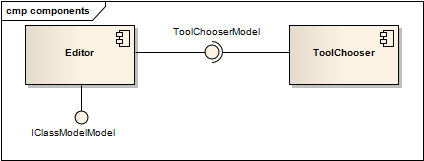
\includegraphics{img/Editor_ToolChooser_Components.png}
\caption{Component diagram of Editor and ToolChooser Modules (created in Enterprise Architect)}
\label{f-Editor_ToolChooser_Components}
\end{center}
\end{figure}

\section{API Module}

This module defines interfaces whose implementations can be found in the lookup of the workspace (workspace is the part of the editor module). Purpose of these interfaces are described in next sections. This module is public so it can be used by any other module (or any other plugin). There are two packages in this module:

\begin{itemize}
    \item cz.cvut.indepmod.classmodel.api.model
    \item cz.cvut.indepmod.classmodel.api.toolchooser
\end{itemize}

\subsection{ClassModel API}
\label{section:classModelAPI}

This package contains interfaces whose implementation can be used to access the information about class model. Lookup of the workspace contains the implementation of the IClassModelModel interface. This object provides the information about the type of a model (business model / class model), list of elements from the model (IElement interface) and the picture of the model. IElement represents a class, an interface or an enumeration. Elements provides the list of annotations (IAnotation interface), attributes (IAttribute interface), methods (IMethod interface) and relations to other classes(IRelation interface). And so on with the attributes, etc. These interfaces represents the structure of the class model meta-model, described in section \ref{classModelMetaModel}.

Relation between (two) classes is represented by instance of IRelation interface. IElement returns the list of IRelations that belongs to it. IRelation holds information about its type (simple relation, composition, agregation, generalization, implementation) and about what element is at the beginning and at the end of the relation, including cardinalities. 

Cardinalities are represented by instance of ICardinality interface. The ICardinality interface has two methods (getFrom() and getTo()) which return from and to value (both are of integer type). Sign of infinity (e.g. in the 1..* or * cardinality) is treated as -1. In the Table \ref{tab:cardinalityExamples} you can see examples of return values of some cardinalities.

\begin{table}[!ht]
\begin{center}
\begin{tabular}{|l|c|c|}
	\hline
	{ \bf Cardinality } & { \bf getFrom() result } & { \bf getTo() result } \\
	\hline \hline
	0 (or 0..0)      & 0 & 0  \\
	1 (or 1..1)      & 1 & 1  \\
   4 (or 4..4)      & 4 & 4  \\
	* (or 0..*)      & 0 & -1 \\
	1..*             & 1 & -1 \\
   0..1             & 0 & 1  \\
   2..5             & 2 & 5  \\
	\hline
\end{tabular}
\caption{Examples of cardinalities}
\label{tab:cardinalityExamples}
\end{center}
\end{table}

The ClassModel API can be treated as a tree. The root node of the tree is IClassModelModel instance whose children are elements, etc. You can see an example of a class diagram in the Figure \ref{f-classApiTree_model} and its tree representation in the Figure \ref{f-classApiTree_tree}.

\begin{figure}[!ht]
\begin{center}
\subfigure[A class diagram]{
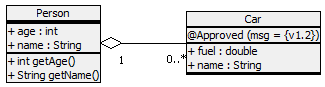
\includegraphics[scale=1]{img/classModelAPITree_model.png}
\label{f-classApiTree_model}
}
\subfigure[A tree representing the class diagram]{
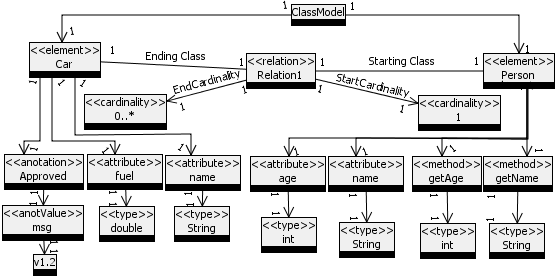
\includegraphics[scale=1]{img/classModelAPITree_tree.png}
\label{f-classApiTree_tree}
}
\caption{Example of ClassModel API Tree}
\label{f-classApiTree}
\end{center}
\end{figure}

\subsection{ToolChooser API}

ToolChooser API is used to hold information about the selected tool of Editor module. The main part of this module is ToolChooserModel class. Instance of this class represents the actual selected tool. ToolChooserModel implements the Observer design pattern so you can register your listener which will be called anytime the model changes.

The API is used by both ToolChooser and Editor modules. Workspace (part of Editor Module) has an instance of ToolChooserModel in it's lookup. This means that Editor module leaves the tool selection on someone else.

ToolChooser uses this instance (from the lookup of active workspace) to set the desired tool (e.g. new class).  But it is also possible to make another plugin that will do this (e.g. in the toolbar). Structure of this package is really simple and you can see it in the Figure \ref{f-ModuleAPIToolChooserModel}.

\begin{figure}[!ht]
\begin{center}
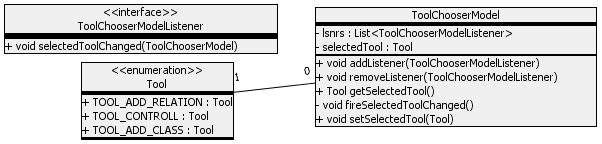
\includegraphics[width=\textwidth]{img/ModuleAPIToolChooserModel.png}
\caption{Class Diagram of ToolChooser API package}
\label{f-ModuleAPIToolChooserModel}
\end{center}
\end{figure}

\section{ToolChooser Module}
\label{section:toolChooserModule}

This module is used for setting of demanded tool of active workspace. The user interface of this module can be seen in the screen shot of the running application (Figure \ref{f-screenSmallModule}).

ToolChooser searches for instance of the ToolChooserModel in the lookup of active workspace (Editor module). When the instance is found, ToolChooser can set its tool (new class, new relation, etc.). This means that it can be used to set the desired tool of that workspace. The structure of this module can be seen in the Figure \ref{f-ToolChooserModuleToolChooser}.

\begin{figure}[!ht]
\begin{center}
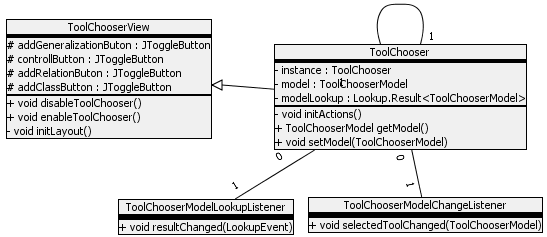
\includegraphics[width=\textwidth]{img/ToolChooserModuleToolChooser.png}
\caption{Class Diagram of ToolChooser Module}
\label{f-ToolChooserModuleToolChooser}
\end{center}
\end{figure}

ToolChooser is a singleton which is inherited from the TopComponent class. TopComponent is provided by Netbeans platform. It is derived from standard JComponent class (javax.swing) and adds many methods which can be used for controlling a window. Ancestors of TopComponent class can be used as a user interface (component that is visible to the user) in the Netbeans platform application. More info can be found in \cite{netbeans6.9DevGuide} in chapter called Window System).

In the layer.xml file there is set the action for opening the ToolChooser (in running application can be accessed in menu Windows \ding{221} Tool Chooser). Layer.xml is a configuration file of the Netbeans platform, which is provided by modules. Content of this file defines new folders and files which will be inserted into the system filesystem (a central registry) when the module is loaded. The system filesystem is a virtual filesystem, which is used for Netbeans platform settings. For example there are some folders that are used for Window System API (window positions, etc.) or Actions API (e.g. actions in the menu) configuration. More info about this can be found in \cite{netbeans6.9DevGuide} in the chapter 3, called Window System.

\section{Editor Module}

This is the fundamental module whose purpose is to create a workspace which provides the class modeling. For graphical part of class modeling is used framework JGraph (\cite{JGraphWeb}). More info about JGraph framework can be found in \cite{jgraphmanual}.

\subsection{Module Structure}
\label{section:editorModuleStructure}

Main class (part of the cz.cvut.indepmod.classmodel.workspace package), which represents the workspace, is the ClassModelWorkspace. Thus, if you want to study the code, you should start right here. ClassModelWorkspace is extended from the TopComponent. This class is responsible for whole initialization. It creates:
\begin{itemize}
    \item ClassModelGraph - this class is extended from JGraph and represents the class model graph to the user. Instance of this class is situated inside the ClassModelWorkspace component (JGraph is also derived from JComponent)
    \item ClassModelModel - Implementation of IClassModelModel which returns the list of classes that are in the class model and the type of the diagram (class or business model). The purpose of IClassModelModel interface is described in the section \ref{section:classModelAPI}.
    \item ClassModelMarqueeHandler - this class is responsible for user input handling which is made inside the ClassModelGraph.
\end{itemize}

ClassModelWorkspace is simply JComponent (TopComponent) which has the JGraph inside. JGraph presents the class model to the user. There are cells (representing classes) which are related together by edges (representing relations).

In the next section I will try to describe the implementation of the Editor Module. I Will start from the initialization and after that I will try to explain every part that is created during the initialization.

\subsection{Editor Module Initialisation}

As I have already said before, the ClassModelWorkspace class does the initialization of the whole module. There are two cases of initialization. The first case, when user creates new class diagram, and the second, when user opens an existing model from file. Both cases are very similar. They differ in the way of DiagramDataModel initialization. For this purpose there are two constructor variants.

The first, non parametric, constructor is used when the new class diagram (with no associated file) is created. This constructor calls the DiagramModelFactory which creates new instance of DiagramDataModel and returns it.

The second constructor is used when the user opens a file with a class model. It accepts an instance of ClassModelXMLDataObject (one parameter). This object represents the file in which is the class model saved (more in the chapter \ref{subsection:fileAssociation}). The constructor gets the input stream of that file and asks the ClassModelXMLCoder to decode its content. ClassModelXMLCoder decodes it and returns DiagramDataModel instance filled according to that file's content. ClassModelXMLCoder is part of the persistence layer and will be discussed in the chapter \ref{subsection:persistence}.

DiagramDataModel class represents the data which has to be persisted when user want to save his class diagram. At present, instance of this class holds the GraphLayoutCache instance (class of JGraph framework which holds the information about cells in the graph), list of static data types (list of default data types, like e.g. String or int, for certain language which is chosen during new class diagram file creation), list of dynamic data types (data types that user created by hand), list of stereotypes and the type of the diagram (class or business model, it is also chosen during new file creation). The DiagramDataModel is also used inside the Editor module, especially by forms. To fulfil the rule of loose coupling, forms does not hold the pointer to it but they gain the pointer through the lookup of active diagram. The lookup will be described later in the section \ref{subsection:lookup}.

After the DiagramDataModel is gained (created or loaded) the initialization is the same. What the ClassModelWorkspace creates have been already written up in the chapter \ref{section:editorModuleStructure}. For better understanding you can see the sequence diagram in the Figure \ref{f-ClassModelWorkspaceInicializationSimple} which shows the initialisation of new ClassModelWorkspace. For simplicity there is only what ClassModelWorkspace creates. The processes inside these classes are not shown (Sequence diagram would have been really big) but the process of creation will be discussed later.

\begin{figure}[!ht]
\begin{center}
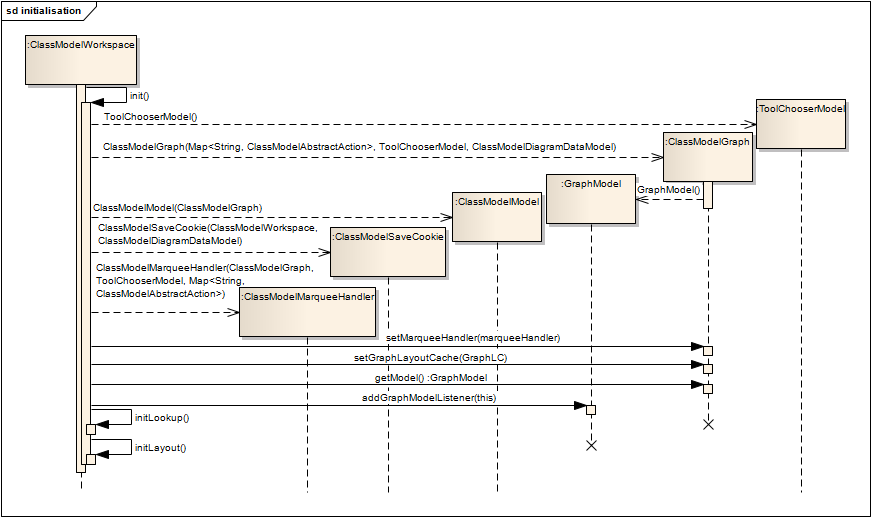
\includegraphics[width=\textwidth]{img/ClassModelWorkspaceInicializationSimple.png}
\caption{Simplified sequence diagram of ClassModelWorkspace initialization}
\label{f-ClassModelWorkspaceInicializationSimple}
\end{center}
\end{figure}

\subsection{ClassModelGraph implementation}

ClassModelGraph is extended from JGraph, which provides a lot of useful functionality (more on this can be found in \cite{jgraphmanual}). ClasModelGraph adds some functionality for class manipulation. This added functionality is shown in following list.
\begin{itemize}
    \item insertCell(Point p) - creates new cell on desired position according to the selected tool (in ToolChooserModel). Usage of this function is shown in the section \ref{subsection:apiImplementation} in Figure \ref{f-ClassCreationSequenceDiagram}.

    \item getAllClasses() - returns the list of classes that are in the diagram. Usage of this function will be shown in the section \ref{subsection:apiImplementation}

    %\item getAllTypes() - returns the list of all data types in the diagram. In addition to the classes (the class is a data type) there are also static data types (like String or int in Java).
\end{itemize} 

To handle events in the graph (ClassModelGraph) there is the ClassModelMarqueeHandler. Instance of this class is created in the ClassModelWorkspace and is added into the ClassModelGraph instance. Purpose of this class is to handle all user inputs in the ClassModelGraph (in the canvas of the graph) and control the popup menu (JPopupMenu and its content). When user does an action (e.g. click with mouse), the ClassModelMarqueeHandler will find out if it is a control click (e.g. cell selection), new cell addition, edge (line between cells) addition and so on. This class is also responsible for rendering of the temporary line when user creates new edge.

\subsection{JGraph class cell rendering}

In this section I will explain how I render the classes (the rectangles with the class name and lists of annotations, attributes and methods) into the JGraph workspace. But first a little theory remind. JGraph uses MVC pattern for cell rendering. Cells (the model of cell) in JGraph are represented by DefaultGraphCell (or its subclasses). DefaultGraphCell implementation stores the user object and an attribute map. The user object is an object which is associated with the cell. The Cell uses its method toString to render the name of the cell, so in most cases this object is an instance of String. But it can be any other object which can store another information about the cell. The attribute map is used when you want to set the appearance of the cell.

All graph cell has an associated view (VertexView implementation). This VertexView implementation associates the renderer, editor and cell handle\footnote{Cell handle is what appears when the cell is selected (e.g mouse click) and what allows to resize it.} together for a cell (DefaultGraphCell implementation). The cell and the view is associated together by CellViewFactory which returns a cell view for a particular cell. More on this theme can be found in \cite{jgraphmanual}.

JGraph basically supports rendering of basic shapes like rectangles, ovals and so on. When you want to render your own shape, you have to create your own cell view (VertexView), renderer (CellViewRenderer) and CellViewFactory implementation.

So this is what I did. I created ClassModelCellViewFactory which is derived from JGraph's DefaultCellViewFactory and overrides it's method createVertexView(Object o). If the object in the parameter is instance of ClassModelClassCell class, the method returns new instance of ClassModelVertexView (derived from JGraph's VertexView). Otherwise the method returns the default view (calls its parent's method). ClassModelVertexView returns instance of ClassModelVertexRenderer which is derived from VertexRenderer. ClassModelVertexRenderer overrides its method getRendererComponent. This method returns new instance of ClassComponent. ClassComponent is extended from JComponent and renders the class according to the ClassModel user object.

These classes can be found in the package cz.cvut.indepmod.classmodel.workspace.cell. Instance of ClassModelCellViewFactory is inserted into the GraphLayoutCache during the workspace initialisation. You can see the class diagram in the Figure \ref{f-ClassModelVertexStructure}.

\begin{figure}[!ht]
\begin{center}
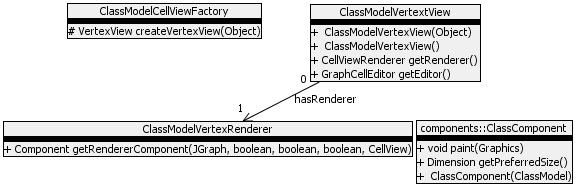
\includegraphics[width=\textwidth]{img/ClassModelVertexStructure.png}
\caption{Structure of classes which render the class cell}
\label{f-ClassModelVertexStructure}
\end{center}
\end{figure}

\subsection{ClassModel API implementation}
\label{subsection:apiImplementation}

Implementation classes of ClassModel API (its interfaces are in the API Module) are situated in the cz.cvut.indepmod.classmodel.cell.model.classmodel package. Main problem I had to deal with was to design where to store the data of the ClassModel.

Basically, ClassModel class is used as a User Object for JGraph cells. User Object (Class Model instance) does not have normally the pointer to its cell (only cell has the pointer to it's User Object). ClassModel holds information like name of the class and list of its attributes, methods and annotations. But where to store the information about relations with other cells (classes)? This information is stored in the JGraph (in its model). So the first idea was to copy this information into the ClassModel instance when an relation is created. But this is not very nice because of data duplication. The second purpose was to add an pointer to cell into the ClassModel instance. But how? The answer is quite simple. I created the ClassModelClassCell which extends DefaultGraphCell of JGraph. The extension of this class is that it adds an pointer to itself into the User Object if this User Object is instance of ClassModel.

So problem is solved. Some information like the name are stored inside the User object and some like the relations are gained from the JGraph cell. In the Figure \ref{f-ClassCreationSequenceDiagram} you can see how is created a class when user selects new class tool in the ToolChooser and clicks somewhere in the ClassModelGraph (JGraph) workspace.

\begin{figure}[!ht]
\begin{center}
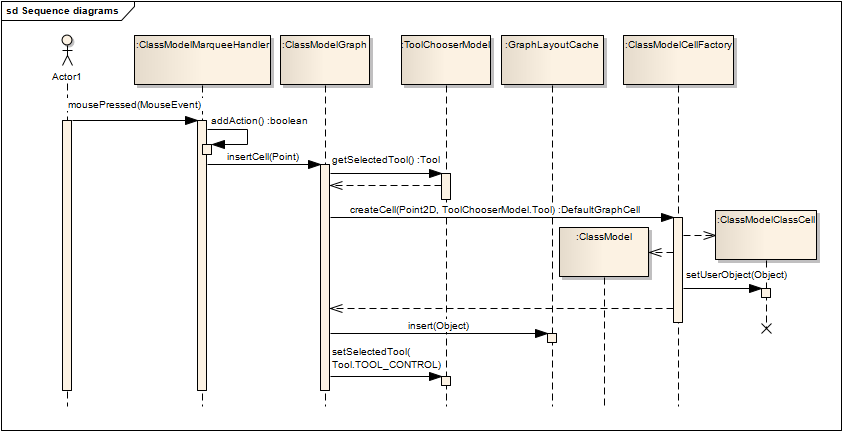
\includegraphics[width=\textwidth]{img/ClassCreationSequenceDiagram.png}
\caption{Sequence Diagram of class creation}
\label{f-ClassCreationSequenceDiagram}
\end{center}
\end{figure}

\subsection{Dialogs}

Dialogs of the Indepmod Class Notation plugin is created on Swing technology. Their classes are located in cz.cvut.indepmod.classmodel.frames.dialogs package.

Every dialog uses the special case of MVC\footnote{MVC - Model View Controller} design pattern. Standard MVC design pattern has three single components:
 \begin{itemize}
    \item a model - represents the data that is processed. It can be e.g. a class instance that holds this data.
    \item a view - presents the data to the user. It is e.g. a form with single components but it does not have to be only the form. It can be also an image or a chart. The view holds the pointer to its model so it can be refreshed when there is a change in the model.
    \item a controller - has a pointer to both the view and the model. It performs an action when user does something (e.g. click on a button in a view) and updates the values in the model.
\end{itemize}

The MVC pattern in this project is slightly different. The view and the controller are not separated but the view is an predecessor of the controller. It is done so because it is not expected to change the view for another else. This does not violate the rule of encapsulation and in addition, the form elements (text fields, buttons, etc.) can be in the view created with protected visibility. It means that the controller can manage these elements directly. You might be asking why is used this amended version of MVC pattern? Answer is, that this project was not created upon the Netbeans API from the beginning. At the beginning, this project was a plugin for a Promod application\footnote{Promod is the application of the master's thesis written by Petr Zv\v{e}\v{r}ina.} and this type of MVC pattern were used.

For better view of the MVC design pattern you can take a look at the Figures \ref{f-classDiagStdMVC} and \ref{f-classDiagIndepmodMVC} where is shown the principle of this design pattern. Detailed info about this design pattern can be found in \cite{DesignPatterns}.

\begin{figure}[!ht]
\begin{center}
\subfigure[Standard MVC Design Pattern]{
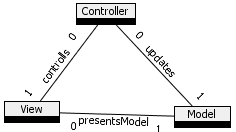
\includegraphics[scale=1]{img/MVCStandard.png}
\label{f-classDiagStdMVC}
}
\subfigure[MVC Design Pattern used in the Indepmod Class Notation]{
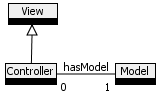
\includegraphics[scale=1]{img/MVCOfIndepmod.png}
\label{f-classDiagIndepmodMVC}
}
\caption{Class diagrams of MVC Design patterns}
\label{f-classDiagMVC}
\end{center}
\end{figure}

Another design pattern that some forms use is the Abstract Factory in conjunction with Template method. The Abstract Factory design pattern solves the problem when we want to create an implementation \textit{A} of an interface under any conditions and another implementation \textit{B} of the same interface under any other conditions. It consists of three parts. The first part is an abstract class which is the abstract factory. This class defines the interface for concrete classes (concrete factories) and a static method which returns an implementation of concrete factory. This static method can accept some parameters from which it decides which concrete factory to return. The second part is consisted of these concrete factories. Their responsibility is to create single components according to the interface of the abstract factory. The third part is consisted of components which are created by these concrete factories.

\begin{figure}[!ht]
\begin{center}
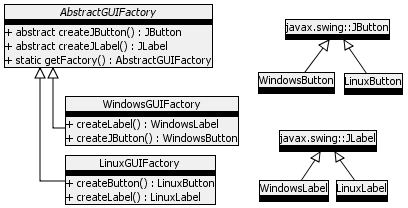
\includegraphics[]{img/AbstractFactoryExample.png}
\caption{Abstract Factory design pattern example}
\label{f-AbstractFactoryExample}
\end{center}
\end{figure}

You can see an example of Abstract factory design pattern in the Figure \ref{f-AbstractFactoryExample}. Imagine that your application will be used on both Windows and Linux and that you want to use different GUI component on these platforms. The solution is depicted in the example. You will create GUI components by use of AbstractGUIFactory. AbstractGUIFactory will find out on which platform the application is running and returns either WindowsGUIFactory or LinuxGUIFactory. Nevertheless, you won't think much about what factory implementation is returned. These concrete factories are returned as their parent class type - AbstractGUIFactory. The only thing you will do is call appropriate method on the returned object which will get you the component you wish. An that is all. For better imagination I will show an example in the Appendix \ref{abstractFactoryCodeExample}.

Usage of this design pattern was necessary because Indepmod Class Notation creates two types of diagrams - class and business diagram. The class diagram lets the user edit all elements of classes (attributes, annotations, methods) but the business diagram lets the user edit only the attributes. When user make the action to edit the class, Indepmod Class Notation shows appropriate dialog according to the type of the model.

Forms that are based on this design pattern are forms for class edition and attribute creation. In this thesis I will explain only the principle of the form for class edition. The form for attribute creation is analogous.

The form for class edition of the business diagram is defined by BusinessModelEditClassDialog class and the form for class edition of the class diagram is defined by ClassModelEditClassDialog. These dialogs have many things in common. This is why they have a common predecessors. These predecessors looks like any other dialog except that they are abstract\footnote{Abstract class - it can't create its instances}. These abstract predecessors are AbstractEditClassDialogView (a view) and AbstractEditClassDialog (a controller). 

The abstract view is able to create the whole UI for class diagram class edition. Component initialization is divided into several protected methods. These methods creates single parts of the UI. Their names are: 

\begin{itemize}
    \item initClassNamePanel - creates the panel for name and stereotype edition
    \item initAnotationPanel - creates the panel for annotation edition
    \item initAttributePanel - creates the panel for attribute edition
    \item initMethodPanel - creates the panel for method edition
\end{itemize}

These methods are treated as template methods so they can be overrode. The abstract controller behaves like any other controller of this program.

The BusinessModelEditClassDialog is extended from the abstract controller and overrides methods that creates annotation and method panels. It overrides them in a way that it returns an null pointer. The abstract view compose its UI of these parts and when a part is null, it is not added there. The ClassModelEditClassDialog does not override any method because all desired functionality is done in its predecessors.

These dialogs are created by an Abstract Factory. The Abstract Factory class is placed in the cz.cvut.indepmod.classmodel.frames.dialogs.factory package and is called AbstractDialogFactory. It has a static method which accepts the type of the diagram and returns an instance of a concrete factory. This concrete factory creates the dialog. Please take a look at the javadoc of this project for more information about the names of methods, etc. For more information about the Abstract Factory design pattern take a look at the \cite{DesignPatterns}.

\subsection{Persistence}
\label{subsection:persistence}

Persistence layer implementation is situated in the cz.cvut.indepmod.classmodel.persistence.xml package. There is a ClassModelXMLCoder class that is created as a singleton. Instance of this class is responsible for encoding and decoding the ClassModelDiagramDataModel instance into or from a stream (InputStream or OutputStream). Its method for encoding, \texttt{encode(ClassModelDiagramDataModel model, OutputStream stream)}, is called by SaveCookie (discussed in the section \ref{subsection:lookup}).

ClassModelXMLCoder uses java.beans.XMLEncoder and java.beans.XMLDecoder. This creates the xml file that represents the steps to create the exactly same object that was encoded. Because XMLEncoder can encode in default only some types of objects, there are some persistence delegates that allow to encode particular object I use. These persistence delegates can be found in the cz.cvut.indepmod.classmodel.persistence.xml.delegate package.

If you want to know more about how XMLEncoder or XMLDecoder works, please take a look at \cite{usingXMLEncoder}.

\subsection{Netbeans File Association}
\label{subsection:fileAssociation}

When you want to open a file that is associated with your application (or with your plugin) in a standard Netbeans way, you have to tell the Netbeans which file type is of you application/plugin. 

Netbeans platform allows its plugins to recognize new types of files. So when you want to associate new file type with your plugin, you can do it easily. The configuration of the file association is, like any other configuration, done via the layer.xml configuration file. If you are not familiar with this, you can find it in \cite{netbeans6.9DevGuide} in the chapter called Data System.

The file type association settings, as have been already written, can be found in layer.xml file. At present there is settings of file type association and settings of wizard that can be used to create new class diagram file. In this wizard user sets the name of the file, type of the diagram and the language (Java, C++, etc.). Files that are associated with this plugin are XML files with .cls suffix. Content of these files will be discussed later.

\subsection{Lookup}
\label{subsection:lookup}

Lookup is (in Netbeans platform) a technique to join more plugins together with loose coupling. On the module level, lookups enable to register a service by its provider and find the service by its consumer in a central repository. On the level of single components (TopComponent), lookups enable to exchange data between this component (provider) and consumers. The main difference between lookup on the module level (service registry) and lookup on the component level is that component does not provide its data by a central registry but by its own lookup object. More reading about this can be found in \cite{netbeans6.9DevGuide} in the chapter called Lookup.

Editor Module uses the Lookup on the component level. ClassModelWorkspace creates its Lookup during the initialization. It adds there an instance of ToolChooserModel and an instance of ClassModelModel.

ToolChooserModel instance is used by ToolChooser Module to set the desired tool. Thanks to this, there can be one ToolChooser component which manages all ClassModelWorkspaces. Of cource, ToolChooserModel instance in the lookup can be used by other plugins also.

ClassModelModel instance implements the IClassModelModel interface and can be also used by other plugins. It provides the Class Model API to the outside world. Thanks to this there can be for example another plugin that will generate the code from the class model of this module.

When user does any change in the model (add new class, new relation between classes, change the attribute of the class or something similar), ClassModelWorkspace inserts a SaveCookie instance into its Lookup. This tells the Netbeans platform that this component is changed and can be saved (save action in File menu is enabled). When user calls this action, the SaveCookie tells the ClassModelXMLCoder to save the GraphLayoutCache into the associated file. When it is done, this SaveCookie implementation is removed from the Lookup, so the Netbeans platform knows that the component does not have to be saved.

\subsubsection{Lookup example}

In this section there is an example of how to obtain the IClassModelModel implementation. Because Editor module uses the lookup on the component level, the IClassModelModel implementation can be accessed only from an active workspace. The example is an action that can be configured (in the layer.xml file) to be placed e.g. in the menu or in the toolbox. The command on line 16 is used to obtain instance of IClassModelModel from the active TopComponent's lookup.

\lstset{language=Java, numbers=left, rulesepcolor=\color{gray}, breaklines=true}
\begin{lstlisting}
package somepackage;

import cz.cvut.indepmod.classmodel.api.model.IElement;
import cz.cvut.indepmod.classmodel.api.model.IClassModelModel;
import java.awt.event.ActionEvent;
import java.awt.event.ActionListener;
import java.util.Collection;
import java.util.logging.Logger;
import org.openide.util.Utilities;

public final class MyAction implements ActionListener {

    @Override
    public void actionPerformed(ActionEvent e) {
        IClassModelModel model;
        model = Utilities.actionsGlobalContext().lookup(IClassModelModel.class);

        if (model == null) {
            // There is no class model, inform the user 
            // that he does not have opened the workspace
            // with a class diagram
        } else {
            // You have a class model, start to do something...
        }
    }
}
\end{lstlisting}

On the line 16, there is a command, that loads the implementation of IClassModelModel from an active workspace. \texttt{Utilities.actionsGlobalContext()} returns the Lookup of the active workspace. Active workspace is the TopComponent which the user is working with. This Lookup instance is consequently asked to return the implementation of the IClassModelModel interface.
